% --- chapter5.tex ---
\chapter{System Implementation}
\label{chap:implementation}

This chapter is presenting all the practical implementation of our project. The system integrates VR interactions, speech processing, conversation handling, auto-tagging, condition analysis, therapy simulation selection, and the post-session evaluation into a coherent workflow. Each component operates independently contributing to an overall system designed to provide personalized interventions.

\section{System Architecture}
This system is following a \textbf{client-server architecture} which is distinguishing clearly between the presentation layer (VR Client) and the data processing layer (Backend). Figure \ref{fig:client_server_architecture} is showing the high-level interaction between these components.

\begin{figure}[H]
\centering
\begin{tikzpicture}[
    node distance=1.5cm,
    % Define styles for a professional look
    font=\small\sffamily,
    box/.style={
        draw=cyan!40!black, 
        top color=cyan!5, 
        bottom color=cyan!10, 
        rounded corners=3pt, 
        align=center, 
        minimum height=1cm, 
        minimum width=3cm,
        drop shadow,
        thick
    },
    server/.style={
        draw=gray!50!black, 
        fill=gray!5, 
        rounded corners=5pt, 
        minimum height=5.5cm, 
        minimum width=7cm, 
        dashed,
        label={[anchor=north]north:Backend Infrastructure}
    },
    db/.style={
        shape=cylinder, 
        shape aspect=0.25, 
        draw=orange!40!black, 
        top color=orange!10, 
        bottom color=orange!20, 
        minimum height=1.5cm, 
        minimum width=2cm, 
        align=center,
        drop shadow,
        thick
    },
    client/.style={
        draw=blue!40!black, 
        top color=blue!5, 
        bottom color=blue!15, 
        rounded corners=3pt, 
        align=center, 
        minimum height=1.5cm, 
        minimum width=3.5cm,
        drop shadow,
        thick
    },
    arrow/.style={->, thick, color=gray!70!black, -{Stealth[scale=1.2]}}
]

    % Client Node
    \node[client] (client) {Client Layer \\ \textbf{Unity VR Frontend}};
    
    % Backend Container
    \node[server, right=2cm of client] (server_box) {};
    
    % Components inside Server
    \node[box, fill=white, below right=-4.5cm and -6.5cm of server_box] (gateway) {API Gateway \\ (FastAPI)};
    
    \node[box, below=0.5cm of gateway] (ai_core) {AI Core Services \\ (Mistral, BERT, T5)};
    
    \node[box, below=0.5cm of ai_core] (logic) {Logic \& Scoring \\ (CNN, Report Gen)};

    % Database
    \node[db, right=1cm of server_box] (mongo) {MongoDB \\ Storage};

    % Connections
    \draw[arrow] (client) -- node[above, font=\footnotesize] {HTTPS / WebRTC} (gateway);
    \draw[arrow] (gateway) -- (ai_core);
    \draw[arrow] (ai_core) -- (logic);
    
    % Database connections
    \draw[arrow] (ai_core) -| (mongo);
    \draw[arrow] (logic) -| (mongo);

\end{tikzpicture}
\caption{High-Level Client-Server System Architecture.}
\label{fig:client_server_architecture}
\end{figure}

\newpage
\section{Hardware and Software Requirements}
Table \ref{tab:sys_reqs} have all the details regarding hardware and software specifications used for this implementation.

\begin{table}[H]
\centering
\renewcommand{\arraystretch}{1.4}
\begin{tabular}{|p{0.25\textwidth}|p{0.7\textwidth}|}
\hline
\rowcolor{gray!15} \textbf{Category} & \textbf{Specification Details} \\ \hline
\multicolumn{2}{|c|}{\textbf{Hardware Requirements}} \\ \hline
\textbf{GPU} & NVIDIA A100 or RTX 4090 (Min. 14GB VRAM, CUDA 7.0+) \\ \hline
\textbf{CPU} & 16-Core Processor (2.5GHz+, 16+ Threads) \\ \hline
\textbf{RAM} & 64GB Recommended (24GB reserved for AI Models) \\ \hline
\textbf{Storage} & 500GB NVMe SSD (Model weights, DB, Logs) \\ \hline
\multicolumn{2}{|c|}{\textbf{Software Requirements}} \\ \hline
\textbf{OS} & Ubuntu 22.04 LTS / Windows Server 2022 \\ \hline
\textbf{Backend Stack} & Python 3.10+, FastAPI, Node.js \\ \hline
\textbf{AI Libraries} & PyTorch, Hugging Face Transformers, LoRA, Scikit-learn \\ \hline
\textbf{Database} & MongoDB Community Edition \\ \hline
\textbf{Frontend} & Unity 3D Engine, C\#, WebRTC \\ \hline
\end{tabular}
\caption{System Hardware and Software Specifications}
\label{tab:sys_reqs}
\end{table}

\section{Core Components and Workflow}
The implementation workflow is consisting of many key stages executed by the special AI models. This section outlines the transformation of user input into outcomes.

\subsection{VR Frontend and User Input}
In frontend users interact with the VR environment to give report primary issue. Audio is captured via the headset microphone and given to the backend. In backend it is transcribed using the \textbf{OpenAI Whisper} service.

\subsection{AI Analysis and Tagging}
Two models are processing the transcribed text.
\begin{enumerate}
    \item \textbf{Mistral-7B (LoRA):} It generates an immediate conversational response.
    \item \textbf{BERT Tagger:} It classifies the text into emotional and behavior labels.
\end{enumerate}

\subsection{Simulation Selection Logic}
Our system uses the provided output from the \textbf{T5-Large Analyzer} to determine the VR intervention. Table \ref{tab:sim_mapping} showing the logic used to combine identified conditions to specific simulations.

\begin{table}[H]
\centering
\renewcommand{\arraystretch}{1.2}
\begin{tabular}{|l|l|l|}
\hline
\rowcolor{gray!15} \textbf{Detected Condition} & \textbf{Recommended Simulation} & \textbf{Therapeutic Goal} \\ \hline
General Anxiety & Nature Walk / Breathing & Relaxation \& Grounding \\ \hline
Phobia / Fear & Controlled Exposure & Desensitization \\ \hline
Negative Self-Talk & CBT Logic Puzzle & Cognitive Restructuring \\ \hline
Panic Attacks & Mindfulness Void & Physiological Regulation \\ \hline
Social Isolation & Virtual Cafe Interaction & Social Skills Practice \\ \hline
\end{tabular}
\caption{Mapping of Conditions to VR Simulations}
\label{tab:sim_mapping}
\end{table}

\section{Processing Logic}

\begin{figure}[H]
\centering
% Adjust the width (e.g., 0.6 or 0.8) depending on how tall the image is
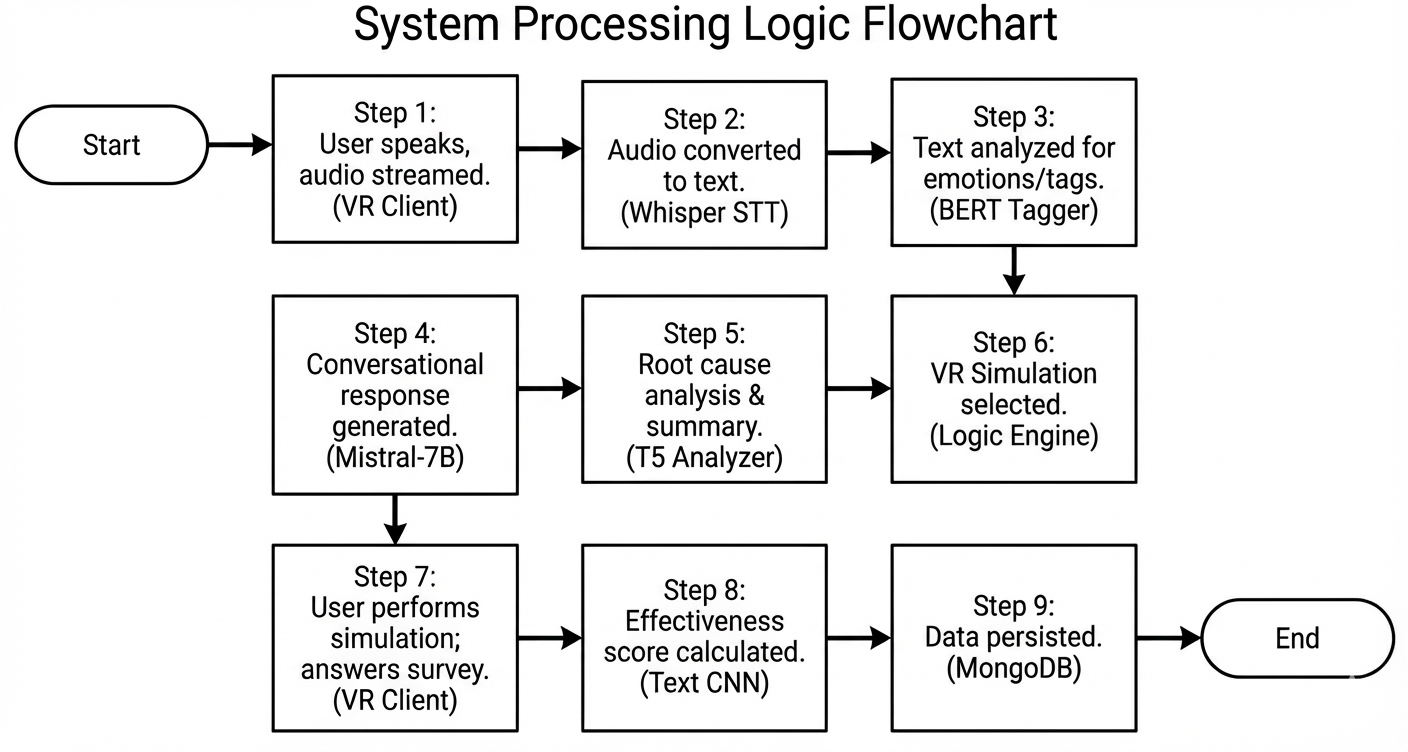
\includegraphics[width=0.8\textwidth]{figures/Processing Logic.png}
\caption{System Processing Logic and Component Interaction}
\label{fig:process_logic}
\end{figure}

\newpage
\section{Data Flow Diagram}
Figure \ref{fig:dfd} given below is visualizing the movement of data through the system. It is highlighting the interactions between the User, the VR ,AI Services, and the Database etc.

\begin{figure}[H]
\centering
\resizebox{\textwidth}{!}{%
\begin{tikzpicture}[
    node distance=2cm,
    font=\sffamily\small,
    box/.style={draw=black, rounded corners, fill=blue!5, align=center, minimum height=1cm, minimum width=3cm, drop shadow},
    ext/.style={draw=black, fill=orange!10, align=center, minimum height=1cm, minimum width=2.5cm, drop shadow},
    db/.style={shape=cylinder, shape aspect=0.2, draw=black, fill=green!10, align=center, minimum height=1.5cm, minimum width=2cm, drop shadow},
    arrow/.style={->, thick, >=Stealth}
]

    % Nodes
    \node[ext] (user) {User};
    \node[box, right=1.5cm of user] (frontend) {VR Frontend};
    
    \node[ext, above=1.5cm of frontend] (stt) {STT (Whisper)};
    \node[ext, below=1.5cm of frontend] (tts) {TTS (ElevenLabs)};
    
    \node[box, right=3cm of frontend] (logic) {Backend Logic};
    \node[box, above=1.5cm of logic] (models) {AI Models\\(Mistral, BERT, T5)};
    \node[db, below=1.5cm of logic] (mongo) {MongoDB};

    % Edges
    \draw[arrow] (user) -- node[above, font=\tiny] {Audio} (frontend);
    \draw[arrow] (frontend) -- node[right, font=\tiny] {Audio} (stt);
    \draw[arrow] (stt) -- node[left, font=\tiny] {Text} (frontend);
    
    \draw[arrow] (frontend) -- node[above, font=\tiny] {JSON Payload} (logic);
    \draw[arrow] (logic) -- node[left, font=\tiny] {Inference} (models);
    \draw[arrow] (models) -- node[right, font=\tiny] {Results} (logic);
    
    \draw[arrow] (logic) -- node[left, font=\tiny] {Store Data} (mongo);
    \draw[arrow] (logic) -- node[below, font=\tiny] {Response} (frontend);
    
    \draw[arrow] (frontend) -- node[left, font=\tiny] {Text} (tts);
    \draw[arrow] (tts) -| node[near start, below, font=\tiny] {Audio Stream} (user);

\end{tikzpicture}%
}
\caption{Data Flow Diagram (DFD) of the Therapy Session}
\label{fig:dfd}
\end{figure}

\section{Deep Learning Model Specifications}
Our system relies on four totally different neural networks. Table \ref{tab:model_summary} is providing an overview of their configurations and roles.

\begin{table}[H]
\centering
\renewcommand{\arraystretch}{1.3}
\resizebox{\textwidth}{!}{%
\begin{tabular}{|l|l|l|l|}
\hline
\rowcolor{gray!15} \textbf{Model Name} & \textbf{Architecture} & \textbf{Parameters} & \textbf{Specific Task} \\ \hline
Mistral-7B & Transformer (LoRA) & 7 Billion & Conversational Empathy \\ \hline
BERT Tagger & Encoder Only & 110 Million & Emotion Classification \\ \hline
T5-Large & Encoder-Decoder & 770 Million & Cause Analysis \& Summarization \\ \hline
Text CNN & Multi-Scale ConvNet & 2 Million & Post-Session Scoring (Regression) \\ \hline
\end{tabular}%
}
\caption{Summary of AI Model Configurations}
\label{tab:model_summary}
\end{table}

\newpage
\subsection{Model 1: Mistral-7B with LoRA (Conversational AI)}
The conversational agent is built on \texttt{Mistral-7B-Instruct-v0.2}. It is finetuned using Low-Rank Adaptation (LoRA) to handle mental health contexts efficiently.

\begin{table}[H]
\centering
\renewcommand{\arraystretch}{1.2}
\begin{tabular}{|l|l|}
\hline
\rowcolor{gray!15} \textbf{Hyperparameter} & \textbf{Value / Setting} \\ \hline
Base Model & \texttt{mistralai/Mistral-7B-Instruct-v0.2} \\ \hline
Fine-tuning Method & LoRA (Low-Rank Adaptation) \\ \hline
LoRA Rank ($r$) & 16 \\ \hline
LoRA Alpha & 32 (Scaling Factor = 2.0) \\ \hline
Dropout & 0.1 \\ \hline
Target Modules & \texttt{q\_proj}, \texttt{v\_proj} \\ \hline
Trainable Parameters & 3.3 Million (0.047\% of total) \\ \hline
Inference Precision & Floating Point 16 (FP16) \\ \hline
\end{tabular}
\caption{Mistral-7B LoRA Configuration}
\label{tab:mistral_config}
\end{table}

\subsection{Model 2: BERT Auto-Tagger (Classification)}
For the categorization of user input into specific emotional states we fine-tuned a BertForSequenceClassification model.

\begin{table}[H]
\centering
\renewcommand{\arraystretch}{1.2}
\begin{tabular}{|l|l|}
\hline
\rowcolor{gray!15} \textbf{Hyperparameter} & \textbf{Value / Setting} \\ \hline
Base Architecture & BERT Base Uncased \\ \hline
Max Input Length & 512 Tokens \\ \hline
Hidden Size & 768 \\ \hline
Attention Heads & 12 \\ \hline
Optimizer & AdamW \\ \hline
Learning Rate & $5 \times 10^{-5}$ (Standard Default) \\ \hline
Batch Size & 16 \\ \hline
Training Loss & 1.5999 \\ \hline
Validation Accuracy & 50.99\% \\ \hline
F1 Score & 0.5255 \\ \hline
\end{tabular}
\caption{BERT Auto-Tagger Configuration}
\label{tab:bert_config}
\end{table}

\newpage
\subsection{Model 3: T5-Large Analyzer (Analysis \& Generation)}
We are using the T5-Large model to generate structured summaries and identify root causes of distress based on the conversation history.

\begin{table}[H]
\centering
\renewcommand{\arraystretch}{1.2}
\begin{tabular}{|l|l|}
\hline
\rowcolor{gray!15} \textbf{Hyperparameter} & \textbf{Value / Setting} \\ \hline
Base Model & \texttt{google/t5-large} \\ \hline
Parameters & 770 Million \\ \hline
Task & Sequence-to-Sequence Generation \\ \hline
Epochs & 3 \\ \hline
Batch Size & 1 (Gradient Accumulation Steps = 8) \\ \hline
Learning Rate & $1 \times 10^{-5}$ \\ \hline
Training Loss & 2.0221 \\ \hline
Evaluation Loss & 1.5718 \\ \hline
\end{tabular}
\caption{T5-Large Analyzer Configuration}
\label{tab:t5_config}
\end{table}

\subsection{Model 4: Advanced Text CNN (Scoring)}
A (CNN) is processing survey responses to output a regression score (0--1).

\begin{table}[H]
\centering
\renewcommand{\arraystretch}{1.2}
\begin{tabular}{|l|l|}
\hline
\rowcolor{gray!15} \textbf{Hyperparameter} & \textbf{Value / Setting} \\ \hline
Architecture Type & Multi-Scale 1D CNN \\ \hline
Embedding Dimension & 256 \\ \hline
Kernel Sizes & [2, 3, 4, 5, 6] (Parallel Convolution) \\ \hline
Filters per Kernel & 128 \\ \hline
Activation Function & ReLU + BatchNorm \\ \hline
Dropout Rate & 0.3 \\ \hline
Output Layer & Sigmoid scaled to range [0, 10] \\ \hline
Optimizer & AdamW (LR = 0.001) \\ \hline
\end{tabular}
\caption{Text CNN Configuration for Scoring}
\label{tab:cnn_config}
\end{table}

\section{Summary}
In this chapter we have discussed the detailed technical implementation of our project. We established the client-server architecture which is defining the interaction between the frontend and the Python-based backend. The hardware and software requirements were specified which are highlighting the GPU resources necessary for the deep learning stack. We broke down the core workflow outlining the step-by-step processing logic. The chapter also provided specifications for the four integrated AI models and visualized the data flow which demonstrates a system capable of delivering real-time interventions.
